% Repository:  https://github.com/chiehrosswang/TRB_LaTeX_tex
%
% Transportation Research Board conference paper template
% version 4.0 Lite (updates made to be compatible in Overleaf and ShareLaTeX)
% 
% 
% When numbered option is activated, lines are numbered.
\documentclass[numbered]{trbunofficial}
\usepackage{graphicx}
\usepackage{cmbright}
\usepackage{amsfonts}
\usepackage{amssymb}
\usepackage{amsmath}
\usepackage{graphics}
\usepackage{graphicx}
\usepackage{color}
\usepackage{subcaption}
\usepackage{tikz}
\usetikzlibrary{fit, positioning, calc, decorations.pathreplacing}
\usepackage[export]{adjustbox}

% \usepackage[colorlinks=true,linkcolor=blue,citecolor=blue]{hyperref}
% For TRB version hide links
\usepackage[hidelinks]{hyperref}

\captionsetup{font={small},skip=0.25\baselineskip}
\captionsetup[subfigure]{font={small}, skip=0.1pt, singlelinecheck=true}

% % Leave first line un-commented to display comments, or second to hide all comments
% \newcommand{\basecomment}[1]{#1}
% % \newcommand{\basecomment}[1]{}
% \newcommand{\mok}[1]{\basecomment{\textcolor{blue}{MOK: #1}}}
% \newcommand{\je}[1]
% {\basecomment{\textcolor{blue}{JE: #1}}}
% \newcommand{\gm}[1]
% {\basecomment{\textcolor{blue}{GM: #1}}}

% Put here what will go to headers as author
\AuthorHeaders{Wei, McDonald, Garcia, Markkula, Engstr\"{o}m, and O'Kelly}
\title{An active inference model of car following: Advantages and applications}

% TODO: add macros for easier formatting of \author.

\author{%
  \textbf{Ran Wei}\\
  \hfill\break
  \textbf{Anthony D. McDonald, Corresponding Author}\\
  \hfill\break%
  \textbf{Alfredo Garcia}\\
  \hfill\break%
  \textbf{Gustav Markkula}\\
  \hfill\break%
  \textbf{Johan Engstr\"{o}m*\footnote{*Advisors}}\\
  \hfill\break%
  \textbf{Matthew O'Kelly*}
}

% If necessary modify the number of words per table or figure default is set to
% 250 words per table
% \WordsPerTable{250}

% If words are counted manually, put that number here. This does not include
% figures and tables. This can also be used to avoid problems with texcount
% program i.e. if one does not have it installed.
% \TotalWords{200}

\begin{document}
\nolinenumbers
\maketitle

\begin{center}\textbf{Abstract}\end{center}%
Driver process models play a central role in the testing, verification, and development of automated and autonomous vehicle technologies. Prior models developed from control theory and physics-based rules are limited in automated vehicle applications due to their restricted behavioral repertoire. Data-driven machine learning models are more capable than rule-based models but are limited by the need for large training datasets and their lack of interpretability, i.e., an understandable link between input data and output behaviors. We propose a novel car following modeling approach using active inference, which has comparable behavioral flexibility to data-driven models while maintaining interpretability. We assessed the proposed model, the Active Inference Driving Agent (AIDA), through a benchmark analysis against the rule-based Intelligent Driver Model, and two neural network Behavior Cloning models. The models were trained and tested on a real-world driving dataset using a consistent process. The testing results showed that the AIDA predicted driving controls significantly better than the rule-based Intelligent Driver Model and had similar accuracy to the data-driven neural network models in three out of four evaluations. Subsequent interpretability analyses illustrated that the AIDA's learned distributions were consistent with driver behavior theory and that visualizations of the distributions could be used to directly comprehend the model's decision making process and correct model errors attributable to limited training data. The results indicate that the AIDA is a promising alternative to black-box data-driven models and suggest a need for further research focused on modeling driving style and model training with more diverse datasets. 

\hfill\break%
\noindent\textit{Keywords}: Driver behavior modeling, Active Inference, Behavior Cloning, Intelligent Driver Model, Car Following, Learning from Demonstration
\newpage

\section{Introduction}
The rapid development of automated and connected vehicle technologies has created a corresponding demand for models of driver behavior that can be used to calibrate design parameters \cite{scheel2022urban, scanlon2021waymo}, evaluate technologies \cite{bargman_counterfactual_2017, roesener2017safe}, and refine real-time decision making \cite{rhinehart2019precog}. To be effective in these tasks, driver models must be flexible, generalizable, and interpretable. Model flexibility is the ability of the model to mimic nuanced social behavior of human drivers \cite{brown2017social}. Generalizability is the ability of the model to extend to new environments with minimal modeler intervention. Interpretability refers to both a clear connection between model mechanics and predicted behavior and a grounding in human psychology \cite{markkula2022explaining}. These elements facilitate model inspection and diagnostics which are essential for interpretable models \cite{raukur2022toward}. Car following is an important driving sub-task as it represents a large portion of current driving time and crashes involving automated vehicles \cite{Alambeigi_trb,novakazi2021levels}. Moreover, it requires a complex expression of social behaviors through physical vehicle positioning \cite{brown2017social}, e.g., speeding up to prevent a vehicle from merging. Therefore, it is important to develop flexible, generalizable, and interpretable car following models for automated vehicles and future transportation systems.

Existing car following models can be partitioned into rule-based models and data-driven models \cite{saifuzzaman2014incorporating,mcdonald2019toward}. Rule-based models generate acceleration behavior based on a function specified by the modeler. Typically, this function is grounded in known observations or driver behavior theory \cite{saifuzzaman2014incorporating}. For example, the Intelligent Driver Model (IDM) predicts driver acceleration based on deviations from a desired speed and distance headway \cite{kesting2009agents}. While rule-based models have a clear connection between model mechanics and predicted behavior, they are limited in their flexibility and generalizability. Because the rules in rule-based models are designed to replicate driving behavior in specific contexts and depict driver characteristics with small parameter sets, they are limited in the behavioral repertoire and in generalizing to scenarios outside of those governed by rules beyond their initial rule set. For example, research has shown that rule-based models designed for car following do not generalize to emergency scenarios and crashes \cite{hamdar2008existing}. Despite these limitations, rule-based models are still widely used for automated vehicle analyses \cite{talebpour2016influence} and thus offer a valid benchmark for new models.

In contrast to rule-based models, data-driven models learn a function mapping observations or features to acceleration behaviors using an algorithm. Recent works have used neural networks \cite{zhou2017recurrent}, hybrid neural network algorithms with physics constraints \cite{mo2021physics}, reinforcement learning \cite{zhu2018human}, and adversarial imitation learning \cite{bhattacharyya2020modeling} to model car following behavior. These approaches have shown considerable flexibility in replicating human behavior, however, data-driven models still struggle to reproduce well-known traffic phenomena such as stop-and-go oscillation and their generalizability is constrained by the chosen machine learning technique \cite{zhou2017recurrent, spencer2021feedback}. Furthermore, the complexity of existing data-driven models prohibits interpretability both in the connection between input and output and in their grounding in human psychology. Despite these shortcomings, data-driven models are more generalizable to complex scenarios which are difficult for manual model specification. One important class of data-driven models is Behavior Cloning (BC) known for their simplicity and general effectiveness \cite{pomerleau1988alvinn, codevilla2019exploring, kumar2021should}. Neural network-based BC models have been widely adopted for developing and evaluating automated vehicle algorithms and are a common benchmark for evaluating novel data-driven models \cite{igl2022symphony, suo2021trafficsim}.

The relative strengths of rule-based and data-driven approaches suggest that there is a role for model structure (to aid in interpretability) --- especially structure grounded in psychological theory \cite{markkula2022explaining} --- and learning from data (to aid in flexibility) in car following model development. The incorporation of these two concepts requires a shift to contemporary theories of human cognition. One relevant theory is active inference \cite{friston2010free, friston2017active} --- a framework developed from Bayesian principles of cognition \cite{doya2007bayesian,gershman2015computational}. The central ideas of active inference are that 1) humans have internal probabilistic generative models of the environment and that 2) humans leverage their model of the environment to make inferences about action courses that reduce surprise in terms of both distance from their desired states of the environment and uncertainty \cite{friston2010free, friston2017active}. Importantly, these principles have been translated into a quantitative framework for modeling human behavior and cognition \cite{friston2017active, smith2021recent}. The quantitative framework includes an explicit representation of agent belief dynamics to facilitate agent decision making and action selection in response to observed perceptual signals. Due to this structure, the model is fundamentally interpretable (i.e., actions can be traced back to beliefs and observations at a given time). On the other hand, the increased complexity and probabilistic nature of the model compared to rule-based frameworks also increase it's flexibility and potentially it's generalizability. Recently, the active inference framework has been extended to driving to depict driving behavior during emergency scenarios with some success \cite{wei2022modeling, engstrom2022modeling}, however, the application to broader scenarios has been limited.

Our goal in this article is to introduce the Active Inference Driving Agent (AIDA), evaluate its flexibility and generalizability relative to rule-based and data-driven benchmarks, and illustrate the interpretability of the model and the resulting insights it provides into car following behavior.

\section{Materials and Methods}
In this section, we introduce a formulation of the benchmarks --- IDM and Behavior Cloning --- then describe our AIDA formulation. We then describe the dataset used for model fitting and the model comparison approach. To simplify notation, we adopt a unifying view of car following models as longitudinal driving control policies which map input signals observed by drivers to a control signal, i.e., the instantaneous longitudinal acceleration. We denote the driver observations (or features in machine learning terminology) at discrete time step $t$ by $o_t$ and the control signal by $a_t$. Using this nomenclature, the most generic class of driver control policies can be described as a probabilistic mapping from the entire history of inputs and controls, denoted by $h_t = \{o_{1:t}, a_{1:t-1}\}$ to the next control signal, i.e., $\pi(a_t|h_t)$. However, the control policy may only depend on the most recent observation as $\pi(a_t|o_t)$. The definition of the control policy is the most significant element that differentiates the IDM, Behavior Cloning, and AIDA. These differences are illustrated in  the computation graphs in Figure \ref{fig:comp_graph} and further described in the subsequent sections.

\begin{figure}[!htb]
\centering
    \begin{subfigure}[]{0.3\linewidth}
    \resizebox{1\columnwidth}{!}{%
    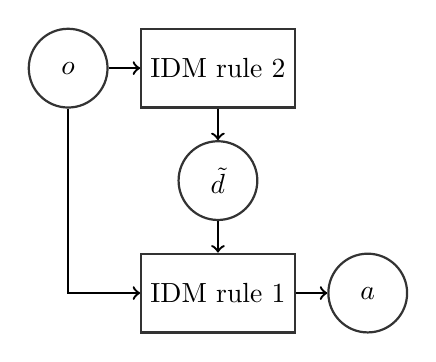
\begin{tikzpicture} 
        \tikzstyle{node}=[circle, draw, minimum size=10mm, thick, draw=black!80, node distance=4mm]
        \tikzstyle{box}=[rectangle, draw, minimum size=10mm, thick, draw=black!80, fill=black!0, node distance=4mm]
        
        \node [box] (f) {IDM rule 2};
        \node [node, left=of f] (x) {$o$};
        \node[node, below=of f] (d) {$\Tilde{d}$};
        \node[box, below=of d] (g) {IDM rule 1};
        \node [node, right=of g] (y) {$a$};
        
        \path [->, line width=0.3mm]
        (x) edge (f)
        (f) edge (d)
        (d) edge (g)
        (g) edge (y);
        \draw [->, line width=0.3mm]
    (x.south) |- (g.west);
    \end{tikzpicture}%
    }
    \caption{IDM}
    \label{}
    \end{subfigure}
    \begin{subfigure}[]{0.3\linewidth}
    \resizebox{1\columnwidth}{!}{%
        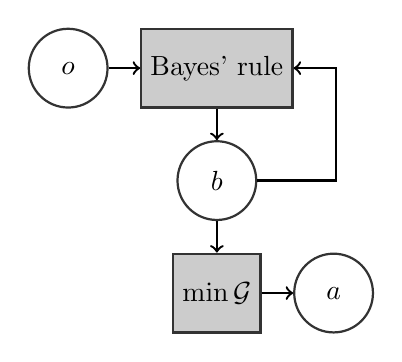
\begin{tikzpicture} 
        \tikzstyle{node}=[circle, draw, minimum size=10mm, thick, draw=black!80, node distance=4mm]
        \tikzstyle{box}=[rectangle, draw, minimum size=10mm, thick, draw=black!80, fill=black!20, node distance=4mm]
        
        \node [box] (f) {Bayes' rule};
        \node [node, left=of f] (x) {$o$};
        \node [node, below=of f] (b) {$b$};
        \node [box, below=of b] (g) {$\min \mathcal{G}$};
        \node [node, right=of g] (y) {$a$};
        
        \path [->, line width=0.3mm]
        (x) edge (f)
        (f) edge (b)
        (b) edge (g)
        (g) edge (y);
        \draw [->, line width=0.3mm]
    (b.east) -- ++(1,0) node(upperleft){} |- (f.east);
    \end{tikzpicture}%
    }
    \caption{AIDA}
    \end{subfigure}
    \begin{subfigure}[]{0.3\linewidth}
    \resizebox{1\columnwidth}{!}{%
        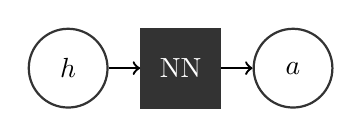
\begin{tikzpicture} 
        \tikzstyle{node}=[circle, draw, minimum size=10mm, thick, draw=black!80, node distance=4mm]
        \tikzstyle{box}=[rectangle, draw, minimum size=10mm, thick, draw=black!80, fill=black!80, node distance=4mm]
        
        \node [box] (f) {\textcolor{white}{NN}};
        \node [node, left=of f] (x) {$h$};
        \node [node, right=of f] (y) {$a$};
        
        \path [->, line width=0.3mm]
        (x) edge (f)
        (f) edge (y);
    \end{tikzpicture}%
    }
    \caption{BC}
    \label{}
    \end{subfigure}
\caption{Computation graphs for (a) IDM, (b) AIDA, and (c) neural network BC models. $o=$ instantaneous observation, $a=$ control action, $h=$ complete interaction history, $\Tilde{d}=$ desired distance headway, $b=$ instantaneous belief, $\mathcal{G}=$ expected free energy, $\text{NN}=$ neural network.}
\label{fig:comp_graph}
\end{figure}

\subsection{Intelligent Driver Model}
The IDM \cite{treiber2000congested} implements a control policy based on drivers' instantaneous observation of their own vehicle's speed $v$, relative speed to the lead vehicle $\Delta v$, and distance headway to the lead vehicle $d$, i.e., $\pi(a_t|o_{t}=\{v_t, \Delta v_t, d_t\})$. At each time step, the IDM computes a longitudinal acceleration to regulate the driver's vehicle towards a desired speed $\Tilde{v}$ and desired distance headway $\Tilde{d}$ using the following control rule:
\begin{align}\label{eq:idm1}
   a_t = a_{max}\left[1 - \left(\frac{v_t}{\Tilde{v}}\right)^{4} - \left(\frac{\Tilde{d}}{d_t}\right)^2\right]
\end{align}
where the desired distance headway is defined as:
\begin{align}\label{eq:idm2}
    \Tilde{d} = d_{0} + v_{t}\tau - \frac{v_t\Delta v_t}{2\sqrt{a_{max}b}}
\end{align}

The IDM has the following parameters: $a_{max}$ the maximum acceleration rate which can be implemented by the driver, $d_0$ the minimum allowable distance headway, $\tau$ the desired headway time, and $b$ the maximum deceleration rate. While these parameters can be set manually by human designers, they usually depend on the road condition and vary with individual driver characteristics, e.g., the desired velocity and minimum distance headway. Thus, various methods have been proposed to calibrate model parameters from traffic data \cite{papathanasopoulou2015towards, treiber2013microscopic}.

A significant limitation of the IDM is that it cannot express certain types of behavior as a result of the control rule defined in (\ref{eq:idm1}) and (\ref{eq:idm2}). For example, it cannot express behavior due to uncertainty about the lead vehicle behavior and surrounding traffic and is limited to modeling behavior in non-conflict scenarios \cite{hamdar2008existing}. Incorporation of such behavior requires significant intervention from the model designers in adapting the control rule, e.g, modifying (\ref{eq:idm1}) and (\ref{eq:idm2}) to depend on additional inputs or ``memory" mechanisms \cite{kesting2009agents}.

\subsection{Behavior Cloning}
BC refers to methods that train neural networks to learn policies from datasets of human car following behavior. The dataset, denoted with $\mathcal{D}$, is usually organized in the form of observation-action trajectories, i.e., $\mathcal{D} = \{o_{1:T}^{(i)}, a_{1:T}^{(i)}\}_{i=1}^{N}$, where $N$ is the total number of trajectories and $T$ is the length of each trajectory. The neural network parameterized policies depend on either the entire history $h_t$ or the most recent observation $o_t$. Let us denote the policy parameters with $\theta$, BC trains policies to maximize the expected log likelihood of the dataset trajectories:
\begin{align}\label{eq:bc_objective}
    \max_{\theta} \mathcal{L}(\theta) = \mathbb{E}_{o_{1:t}, a_{1:t} \sim \mathcal{D}}\left[\sum_{t=1}^{T} \log \pi_{\theta}(a_t|h_t)\right]
\end{align}
BC is simple to implement and more computationally efficient than comparative data-driven machine learning methods like reinforcement learning and online imitation learning. BC also does not require a high fidelity traffic simulation environment for training, which is necessary for reinforcement learning and online imitation learning. In contrast to rule-based policies, BC policies are more flexible and can express a much larger class of behaviors. 

However, BC as a representative offline learning method has known disadvantages of being sensitive to the quantity and quality of training data and input features. The covariate-shift between the training dataset and the testing environment and neural network models' difficulty of extrapolating learned mechanisms to unseen inputs often cause BC models to overfit to the training dataset while producing poor control behavior during closed-loop testing (defined in section \ref{sec:online_test}) \cite{ross2010efficient, spencer2021feedback}. Furthermore, several studies have found that BC can be highly sensitive to input features \cite{bhattacharyya2020modeling, de2019causal, zhou2017recurrent}. Specifically, when a driver's previous control actions are used as input features to the trained policy, it is likely that the policy merely repeats those controls actions in closed-loop testing. This has been interpreted as a form of learning spurious correlations or causal confusion in machine learning, since driver controls at adjacent time steps are usually so similar that predicting previous controls can quickly minimize training error \cite{de2019causal}. Because BC does not impose any structure on the policy, examining the failure modes of BC models is as challenging as examining any other black-box neural network models.

Despite these shortcomings, BC, or variations of it, is a widely studied approach in developing automated vehicle algorithms and building simulated agents and environments for training them \cite{suo2021trafficsim, igl2022symphony}. It can produce high quality simulated behavior in practice when the training dataset is large and diverse, appropriate features are selected, and the neural network model is large and expressive enough \cite{codevilla2019exploring, zhou2017recurrent, kumar2021should} and thus it represents a valid data-driven modeling benchmark. 

\subsection{Active Inference Driving Agent}
An active inference agent is defined by its internal generative model, which we implemented as a Partially Observable Markov Decision Process (POMDP). A POMDP describes a dynamic process in which the state of the environment $s_t \in \mathcal{S}$ evolves with driver actions, $a_t \in \mathcal{A}$, according to a probability distribution, $P(s_{t+1}|s_t, a_t)$, and generates observation signal, $o_{t+1} \in \mathcal{O}$, according to, $P(o_{t+1}|s_{t+1})$. In this work, we assume the observation signals are multivariate continuous variables and the states are discrete to represent probabilistic categorizations of the observation space (i.e., categorical perception \cite{beer2003dynamics}). At every time step, the active inference agent first makes inference about the hidden state of the environment upon receiving observations using Bayes' rule:
\begin{align}\label{eq:aif_belief}
    b_t(s_t) = \frac{P(o_t|s_t)P(s_t|b_{t-1}, a_{t-1})}{\sum_{s_t}P(o_t|s_t)P(s_t|b_{t-1}, a_{t-1})}
\end{align}
where $b_t(s_t) = P(s_t|h_t)$ denotes the agent's belief about the environment state given the observation-action history $h_t$ and $P(s_t|b_{t-1}, a_{t-1}) = \sum_{s_{t-1}}P(s_t|s_{t-1}, a_{t-1})b(s_{t-1})$ is the prior predictive distribution based on the previous belief.

The active inference agent then selects control actions to minimize a criterion known as the (cumulative) expected free energy (EFE) \cite{friston2021sophisticated}:
\begin{align}
    \mathcal{G}^{*}(b_t) = \min_{\pi} \mathbb{E}\left[\sum_{t}^{t+H} EFE(b_t, a_t) + \log \pi(a_t|b_t)\right]
\end{align}
where $H \leq \infty$ is a finite planning horizon. The EFE is defined as:
\begin{align}\label{eq:efe}
    EFE(b_t, a_t) \triangleq \mathbb{E}[D_{KL}\left(b_{t+1}||\Tilde{P}\right)] + \mathbb{E}[\mathcal{H}(o_{t+1})]
\end{align}
where $\Tilde{P} := \Tilde{P}(s_{t+1})$ defines the agent's preferred state distribution, $D_{KL}(\cdot || \cdot)$ denotes the Kullback-Leibler divergence --- measuring the discrepancy between the current belief and the preferred state distribution --- and $\mathcal{H}(\cdot)$ denotes Shannon entropy --- measuring uncertainty about observations. These terms represent goal-seeking and information-seeking (epistemic) behavior respectively \cite{tschantz2020learning}. The first expectation in the EFE is taken with respect to:
\begin{align}\label{eq:predictive}
\begin{split}
    P(o_{t+1}|b_t, a_t) &= \sum_{s_{t+1}}P(o_{t+1}|s_{t+1})P(s_{t+1}|b_t, a_t)
\end{split}
\end{align}
and the second expectation in the EFE is taken with respect to $P(s_{t+1}|b_t, a_t)$. 

Let $\mathcal{G}^{*}(b_t, a_t)$ be defined as:
\begin{align}\label{eq:cumulative_efe}
    \mathcal{G}^{*}(b_t, a_t) := EFE(b_t, a_t) + \log \pi(a_t|b_t) + \int_{}P(o_{t+1}|b_t, a_t)\mathcal{G}^{*}(b_{t+1})d_{o_{t+1}}
\end{align}
Then the optimal policy has a closed-form expression \cite{haarnoja2018soft}:
\begin{align}\label{eq:aif_policy}
    \pi(a_t|b_t) = \frac{e^{-\mathcal{G}^{*}(b_t, a_t)}}{\sum_{\Tilde{a} \in \mathcal{A}}e^{-\mathcal{G}^{*}(b_t, \Tilde{a})}}
\end{align}

Active inference has two important differences from the traditional notion of POMDP in operations research and reinforcement learning. First, both the generative model and the control objective are internal to the agent, meaning they can differ in substantial ways from the true environment generative model or a canonical notion of desired behavior, e.g., a "good driver" should always be centered in the lane. This has important implications as many human driving behaviors can be explained as inference in subjective or sub-optimal models \cite{schwartenbeck2015optimal}. Second, active inference makes an explicit distinction between pragmatic and epistemic behavior in its policy objective according to the first and second terms in (\ref{eq:efe}). This distinction supports adaptive behavior in unknown and uncertain environments \cite{tschantz2020learning, engstrom2018great}, e.g., traffic environments. 

\subsection{Dataset}
We performed our analysis of the IDM, BC, and AIDA using the INTERACTION dataset \cite{zhan2019interaction}, a publicly available driving dataset recorded using drones on fixed road segments in the USA, Germany, and China. The dataset provides a lanelet2 format map \cite{poggenhans2018lanelet2} and a set of time-indexed trajectories of the positions, velocities, and headings of each vehicle in the scene in the map's coordinate system at a sampling frequency of 10 Hz, and the vehicle's length and width for each road segment. The dataset contains a variety of traffic behaviors, including car following, free-flow traffic, and merges. 

Due to our emphasis on car following behavior, we selected a subset of the data to include car following data from a two-way, seven-lane highway segment in China with a total distance of 175 m. We focused on vehicles in the middle two west-bound lanes shown in Figure \ref{fig:map}. We further filtered the remaining vehicles according to two criteria: 1) there was a lead vehicle with a maximum distance headway of 60 m, and 2) the ego vehicle was not performing a merge or lane change. We identified merging and lane change behavior using an automated logistic regression-based approach and validated the classifications with a manual review of a subset of trajectories. We also removed all trajectories with length shorter than 5 seconds, leaving a total of 1,254 trajectories with an average length of 14 seconds.

\begin{figure}
    \centering
    \includegraphics[width=0.8\textwidth]{fig/map.png}
    \caption{Map of the roadway included in data collection. The westbound lanes (blue) were used for training and the eastbound lanes (orange) were used for testing.}
    \label{fig:map}
\end{figure}

\subsubsection{Feature Computation}
The input features to the IDM are defined in (\ref{eq:idm1}) and (\ref{eq:idm2}). For BC and the AIDA, we used $d$ and $\Delta v$ but excluded $v$ to prevent learning spurious correlations to ego speed or acceleration from past time steps reported in prior studies \cite{de2019causal, codevilla2019exploring, zhou2017recurrent}. Furthermore, we included an additional feature $\tau^{-1}$ in BC and AIDA defined as the rate of change of the visual angle of the lead vehicle from the ego driver's seat position divided by the angle itself. $\tau^{-1}$ can be considered as a perceptual-control analog of inverse time-to-collision, a feature commonly used in driver modeling \cite{bhattacharyya2020modeling, svard2021computational,engstrom2018simulating}, with the difference of incorporating the width of the lead vehicle into feature computation and using quantities that can actually be observed by the driver. This is consistent with recent findings on the impact of optical expansion of the lead vehicle's image on driver longitudinal control behavior \cite{markkula2016farewell}. Furthermore, the inclusion of this feature puts the information contained in the inputs to BC and the AIDA on a similar level to the IDM, as the IDM implicitly accounts for time-to-collision in its desired distance headway computation in (\ref{eq:idm2}).

We computed all features in the Frenet frame (i.e., lane-centric coordinates \cite{werling2010optimal}), by first transforming vehicle positions, velocities, and headings using the current lane center line as the reference path and then computing the features from the transformed positions and velocities. We obtained the drivers' instantaneous longitudinal control inputs (i.e., accelerations) from the dataset by differentiating the Frenet frame longitudinal velocities. For BC and the AIDA, we discretized the continuous control inputs into discrete actions using a Gaussian mixture model of 15 Gaussian components with mean and variance parameters chosen using the Bayesian Information Criteria \cite{murphy2012machine}.

\subsection{Model implementation}
In this section, we describe our approach for parameterizing the IDM, BC, and the AIDA. 

\textbf{IDM.} Following \cite{jung2022gray}, we parameterized the IDM by treating the IDM policy as a conditional Gaussian distribution: $\pi(a_t|o_t=\{v_t, \Delta v_t, d_t\}) = \mathcal{N}(a_t|\mu_t, \sigma^2)$ with mean action $\mu_t$ and variance $\sigma^2$. The mean action $\mu_t$ is computed from the IDM rule defined in (\ref{eq:idm1}) and (\ref{eq:idm2}) by making the desired speed $\Tilde{v}$, minimum distance headway $d_0$, desired headway time $\tau$, maximum acceleration rate $a_{max}$ and maximum deceleration rate $b$ adjustable parameters. The action variance $\sigma^2$ is assumed to be independent of the input features and also estimated from data. 

\textbf{BC.} We implemented the BC model with two types of neural network policies: standard Multi-Layer Perceptron (MLP) networks and recurrent neural networks (RNN) following \cite{bhattacharyya2020modeling}. The MLP network takes as input the observation vector (normalized by training set statistics) and outputs a probability distribution over the discrete control actions. The RNN addresses the possibility that driver behavior may be influenced by the full observation history rather than just the most recent observation. For the RNN, we combined a Gated Recurrent Unit (GRU) network \cite{chung2014empirical} with a MLP network, where the GRU network compresses the observation history into a fixed length vector, which is then transformed into the action distribution by the MLP network.

\textbf{AIDA.} We modeled the discrete state transition probabilities $P(s_{t+1}|s_t, a_t)$ and the desired state distribution $\Tilde{P}(s_t)$ of the AIDA using categorical distributions parameterized by their logits. We parameterized the observation distributions $P(o_t|s_t)$ using Normalizing Flow, a flexible class of neural network-based density estimator \cite{rezende2015variational, papamakarios2021normalizing}. This provides the AIDA with adequate flexibility in modeling complex and nonlinear observation sequences and associating observed actions with agent beliefs. Normalizing Flow uses invertible neural networks to transform simple distributions, e.g., Gaussian distributions, into complex and correlated distributions while maintaining the tractability of likelihood evaluation and sampling. In this work, we used a single, shared Inverse Autoregressive Flow \cite{kingma2016improved} to transform a set of conditional Gaussians with mean vector $\mu(s_t)$ and covariance matrix $\Sigma(s_t)$. We modeled a distribution over the agent's planning horizon using a Poisson rate parameter and used the QMDP method \cite{littman1995learning, karkus2017qmdp} as a closed-form approximation of the cumulative expected free energy in (\ref{eq:cumulative_efe}). We approximately computed the entropy of the state-conditioned observation distributions required in the EFE calculation using the entropy of the Normalizing Flow base distributions. In subsequent sections, we refer to the transition and observation parameters with $\theta_1$, the desired state distribution and planning horizon parameters with $\theta_2$, and the combined parameters with $\theta = \{\theta_1, \theta_2\}$. 

We provide additional implementation details in Appendix \ref{sec:appendix}. Our software implementation is publicly available at \cite{wei2022interactive}. 

\subsection{Parameter Estimation}
We estimated the parameters of the IDM, BC, and AIDA by maximizing the expected log likelihood of driver control inputs from the dataset under the corresponding control policy, i.e., (\ref{eq:bc_objective}). This procedure for the AIDA differs slightly from the IDM and BC by requiring a nested step. Between each parameter update in the nested procedure, we first computed the sequence of beliefs given the observation-action history using (\ref{eq:aif_belief}) and the optimal belief-action policy using (\ref{eq:aif_policy}). We then evaluated the log likelihood as a function of the computed beliefs:
\begin{align}\label{eq:aif_objective}
    \max_{\theta} \mathbb{E}_{o_{1:T}, a_{1:T} \sim \mathcal{D}}\left[ \sum_{t=1}^{T-1}\log \pi_{\theta}(a_{t}|b_{t,\theta_1})\right] \quad \text{{\small s.t.}} \quad  \pi_{\theta}(a_t|b_t) = \frac{e^{-\mathcal{G}_{t, \theta}^*(b_t, a_t)}}{\sum_{\Tilde{a}_t \in \mathcal{A}}e^{-\mathcal{G}_{t, \theta}^*(b_t, \Tilde{a}_t)}}
\end{align}

While (\ref{eq:aif_objective}) allows us to learn task-relevant beliefs in active inference agents as it depends on both $\theta_1$ and $\theta_2$, the parameters are fundamentally unidentifiable since there are potentially infinite sets of $\theta$ with the same likelihood \cite{reddy2018you, armstrong2017impossibility, bouchard2004tradeoff}. This is because, for example, the estimation algorithm cannot differentiate between drivers who desire small distance headway and drivers who believe the distance headway will increase to desired levels in subsequent time steps. A possible consequence of this is learning an environment model that deviates significantly from the reality, which leads to a large number of crash or inaction as a result of the agent not being able to recognize the actual environment state \cite{wei2022world}.

In order to constrain the hypothesis space and avoid configurations of $\theta$ that are incompatible with real-world constraints, we designed a data-driven prior distribution $P(\theta)$ encoding likely configurations of $\theta$. Specifically, the prior is defined as $P(\theta) = P(\theta_1)P(\theta_2|\theta_1)$, where:
\begin{align}\label{eq:aif_prior}
    P(\theta_1) \propto \exp\left(\lambda \mathbb{E}_{o_{1:T}, a_{1:T} \sim \mathcal{D}}\left[\sum_{t=1}^{T}\log P_{\theta_1}(o_t|h_{t-1}, a_{t-1})\right]\right)
\end{align}
with hyperparameter $\lambda$ controlling how much the prior distribution prefers model accuracy, measured by expected log likelihood of observations. We let $P(\theta_2|\theta_1)$ be a uniform distribution. In our experiments, we only compute the Maximum A posteriori (MAP) estimate of the Bayesian model by converting the prior into the following loss function added to the objective in (\ref{eq:aif_objective}):
\begin{align}
    \mathcal{L}(\theta_1) = \lambda \mathbb{E}_{o_{1:T}, a_{1:T} \sim \mathcal{D}}\left[\sum_{t=1}^{T}\log P_{\theta_1}(o_t|h_{t-1}, a_{t-1})\right]
\end{align}
To prevent learning unreasonably large observation variance as a result of the observation entropy term in (\ref{eq:efe}), another symptom previously reported in \cite{wei2022world}, we applied a penalty on the $l^2$ norm of the observation covariance parameters. 

Using these prior loss functions, the AIDA MAP estimate can be written as:
\begin{align}
    \theta^{\text{MAP}} = \arg\max_{\theta} \sum_{t=1}^{T}\mathbb{E}_{o_{1:T}, a_{1:T} \sim \mathcal{D}}\left[\log \pi_{\theta}(a_t|b_{t,\theta_1}) + \lambda_1\log P_{\theta_1}(o_t|h_{t-1}, a_{t-1})\right] + \lambda_2\sum_{s}||\Sigma_{\theta_1}(s)||^{2}
\end{align}

\subsection{Model selection}
We trained each model with 15 random seeds controlling model parameter initialization and dataset mini-batch iteration orders. To select the hyperparameters for the AIDA, we first set $\lambda_2=0.1$ since it's sufficient to mitigate overly large covariances. We then trained the model for $\lambda_1 = [0.2, 1, 4]$ and selected $\lambda_1 = 1$ as it best trades off environment model accuracy and agent behavior predictive performance (with criteria described in the next section). 

\subsection{Model Evaluation and Comparison}
We evaluated and compared our models' ability to generate behavior similar to the human drivers in the dataset using both open-loop offline predictions and closed-loop online simulations. In both cases, we evaluated the models on two different held-out testing datasets. The first dataset includes vehicles from the same lanes as the training dataset. This dataset tests whether the models can generalize to unseen vehicles in the same traffic condition. We obtained this dataset by dividing all selected trajectories in the westbound lanes using a 7-3 train-test ratio. The second dataset includes vehicles from the top two eastbound lanes in Figure \ref{fig:map}. This dataset tests whether the models can generalize to unseen vehicles in novel traffic conditions, since the traffic in the eastbound lanes have on average higher speed and less density. We refer to these two datasets as \textit{same-lane} and \textit{new-lane}, respectively. We randomly selected 100 trajectories with a minimum length of 10 seconds from the same-lane dataset and 75 trajectories with a minimum length of 5 seconds from the new-lane dataset for testing.

\subsubsection{Offline Evaluation}
The goal of the offline evaluation was to assess each model's ability to predict a driver's next action based on the observation-action history recorded in the held-out testing dataset. This task evaluates the models' ability to be used as a short-horizon predictor of other vehicles' behavior in an on-board trajectory planner \cite{sadigh2016planning}. We measured a model's predictive accuracy using Mean Absolute Error (MAE) of the predicted control inputs (unit=$m/s^2$) on the held-out testing datasets. For the IDM, we calculated the predicted control inputs by sampling from the Gaussian policy. For BC and the AIDA, we first sampled a discrete action from the action distribution predicted by the models and then sampled from the corresponding Gaussian component in the Gaussian mixture model used to perform action discretization.

\subsubsection{Online Evaluation}\label{sec:online_test}
Rather than predicting instantaneous actions, the goal of the online evaluation was to assess the models' ability to generate trajectories similar to human drivers such that they can be used as simulated agents in automated vehicle training and testing environments \cite{igl2022symphony}. This is fundamentally different from offline predictions because the models need to choose actions based on observation-action history generated by its own actions rather than those stored in the fixed, offline dataset. This can introduce significant covariate shift \cite{spencer2021feedback} sometimes resulting in situations outside of the model's training data, which can lead to poor action selection. 

We built a single-agent simulator where the ego vehicle's longitudinal acceleration is controlled by the trained models and its lateral acceleration is controlled by a feedback controller for lane-centering. The lead vehicle simply plays back the trajectory recorded in the dataset. Other vehicles do not have any effect on the ego vehicle, given our observation space does not contain other vehicle related features. 

Following \cite{suo2021trafficsim}, We measured the similarity between the generated trajectories and the true trajectories using the following metrics:
\begin{enumerate}
    \item Average deviation error (ADE; unit=$m$): deviation of the Frenet Frame longitudinal position from the dataset averaged over all time steps in the trajectory.
    \item Lead vehicle collision rate (LVCR; unit=$\%$): percentage of testing trajectories containing collision events with the lead vehicle. A collision is defined as an overlap between the ego and lead vehicles' bounding boxes. 
\end{enumerate}

\subsubsection{Statistical Evaluation}
Following the recommendations in \cite{colas2019hitchhiker, agarwal2021deep} for evaluating learned control policies, we represented the central tendency of a model's offline prediction and online control performance using the interquartile mean (IQM) of the offline MAEs and online ADEs. Note however for collision rate, we compute the regular mean instead of IQM to account for the collision rate lower bound of 0. The IQMs are computed by 1) ranking all tested trajectories by their respective performance metrics and 2) computing the mean of the performance metrics ranked in the middle 50\%. To compare the central performance difference between the AIDA and baseline models, we performed two-sided Welch's t-tests with 5 percent rejection level on the MAE-IQM and ADE-IQM values computed from different random seeds with the assumption that the performance distributions between two models may have different variances \cite{colas2019hitchhiker, agarwal2021deep}.

\section{Results and Discussion}
\subsection{Offline Performance Comparison}
Figure \ref{fig:offline_mae} shows the offline evaluation results for each model with the model type on the x-axis and the IQMs of acceleration prediction MAEs averaged across the testing dataset on the y-axis. The color of the points in the figure represents the testing condition and each point corresponds to a random seed's result. The points are randomly distributed around each x-axis label for clarity. Dispersion on the y-axis indicates sensitivity in the model to initial training conditions. The plot illustrates that the AIDA had the lowest MAE-IQM in the same-lane tests, followed by BC-RNN, BC-MLP, and IDM. The corresponding pairwise Welch's t-test results in Table \ref{tab:offline_eval} show that these differences are significant. In the new-lane tests, both the AIDA and neural network BC models significantly outperformed IDM. The AIDA performance has higher variance than BC models, however the difference in the central tendency was not significant. These results show that in the current car following setting, the AIDA and BC generalized better to the new-lane scenario than the IDM, mostly likely due to the IDM rules being unable to adapt to different traffic speed and density than the training dataset. The stronger predictive performance in the AIDA and BC-RNN in the same-lane data can be attributed to the fact that driver acceleration actions depend on the full history of past observations rather than just the most recent observation, which can be modeled by the recurrent structure of the AIDA and BC-RNN. The figure also shows that for the same-lane tests, the AIDA had more variance across the random seeds compared to other models, suggesting that it is the most sensitive to local optima in the training process.

\begin{figure}[!htb]
\centering
\includegraphics[width=0.6\textwidth]{fig/offline_mae.png}
\captionof{figure}{Offline evaluation MAE-IQM. Each point corresponds to a random seed used to initialize model training and its color corresponds to the testing condition of either same-lane or new-lane.}
\label{fig:offline_mae}
\end{figure}

\begin{table}[h!]
\caption{Two-sided Welch's t-test results of offline MAE-IQM against baseline models. Asterisks indicate statistical significance with $\alpha=0.05$.}
\label{tab:offline_eval}
\centering
\begin{tabular}{llcc}
\hline
Baseline & Comparison & t(df=14) & p-value \\ \hline
IDM      & same-lane  & t=37.58 & p\textless{}0.001* \\
BC-MLP   & same-lane  & t=32.38 & p\textless{}0.001* \\
BC-RNN   & same-lane  & t=17.31 & p\textless{}0.001* \\
IDM      & new-lane   & t=33.21 & p\textless{}0.001* \\
BC-MLP   & new-lane   & t=0.35 & p=0.73             \\
BC-RNN   & new-lane   & t=-0.12 & p=0.90             \\ \hline
\end{tabular}
\end{table}

\subsection{Online Performance Comparison}
Figure \ref{fig:online_mae} shows the IQM of each model's ADEs from data set trajectories in the online evaluations using the same format as the offline evaluation results. In the same-lane testing condition, all models had an ADE-IQM values between 1.8 m and 2.8 m, which is less than the length of a standard sedan ($\approx$ 4.8 m; \cite{sedan}). Among all models, BC-MLP achieved the lowest ADE values for both the same-lane and new-lane conditions, followed by the AIDA, IDM, and BC-RNN. Furthermore, both the AIDA and BC models achieved lower ADE-IQM in the new lane settings compared to the same-lane setting, however the IDM achieved higher ADE-IQM in the new-lane setting. The Welch's t-test results in Table \ref{tab:online_eval} show that AIDA's online test performances are significantly different from all baseline models in both the same-lane and new-lane settings (P $\leq$ 0.01). These findings confirm that the AIDA and BC models generalized better to the new-lane setting than the IDM and suggest that the AIDA's average online trajectory-matching ability is significantly better than IDM and BC-RNN, although BC-MLP is significantly better than the AIDA.

\begin{figure}[!htb]
\centering
\includegraphics[width=0.6\textwidth]{fig/online_mae.png}
\captionof{figure}{Online evaluation ADE-IQM. Each point corresponds to a random seed used to initialize model training and its color corresponds to the testing condition of either same-lane or new-lane.}
\label{fig:online_mae}
\end{figure}

\begin{table}[h!]
\caption{Two-sided Welch's t-test results of online ADE-IQM against baseline models. Asterisks indicate statistical significance with $\alpha=0.05$.}
\label{tab:online_eval}
\centering
\begin{tabular}{lllc}
\hline
Baseline & Comparison & t(df=14) & p-value \\ \hline
IDM      & same-lane  & t=3.05 & p\textless{}0.01* \\
BC-MLP   & same-lane  & t=-5.46 & p\textless{}0.001* \\
BC-RNN   & same-lane  & t=8.73 & p\textless{}0.001* \\
IDM      & new-lane   & t=58.18 & p\textless{}0.001* \\
BC-MLP   & new-lane   & t=-3.77 & p\textless{}0.001* \\
BC-RNN   & new-lane   & t = 6.87 & p\textless{}0.001* \\ \hline
\end{tabular}
\end{table}

Figure \ref{fig:online_cr_lv} shows the lead vehicle collision rates for each random seed and model using the same format as Figure \ref{fig:online_mae}. The figure illustrates that in the same-lane condition, the random seeds for BC-MLP, BC-RNN, and the AIDA had more collisions than the IDM (0\% collision rate across all seeds). In particular, BC-RNN and the AIDA had substantial differences across random seeds compared to the other models. However, the minimum collision rates for BC-MLP, BC-RNN, and the AIDA were consistent (less than or equal to 1\%). In the new-lane condition, the collision rate was 0\% for all four models. The higher collision rates in the same-lane data are likely due to the traffic density and complexity, which were higher in the same-lane condition compared to the new-lane condition. 

\begin{figure}[!htb]
\centering
    \includegraphics[width=0.6\textwidth]{fig/online_cr_lv.png}
    \captionof{figure}{Lead vehicle collision rate in online evaluation. Each point corresponds to a random seed used to initialize model training and its color corresponds to the testing condition of either same-lane or new-lane.}
    \label{fig:online_cr_lv}
\end{figure}

\subsection{AIDA Interpretability Analysis}
The previous sections suggest that the AIDA can capture driver car following behavior significantly better than the IDM and comparably to data-driven BC models. However, the findings have yet addressed the interpretability of the AIDA. While there is no established metric for model interpretability, R{\"a}ukur et. al. \cite{raukur2022toward} recommend assessments based on the easiness of comprehending the connection between model input and output and tracing model predictive errors to internal model dynamics. Given that the AIDA's decisions are emitted from a two-step process, i.e., (1) forming beliefs about the environment and (2) selecting control actions that minimize free energy, the model's success at the car following task depends on the two sub-processes both independently and jointly. We examined the AIDA's learned input-output mechanism by visualizing its independent components (i.e., the observation, transition, and preference distributions) and verified them against expectations guided by driving theory \cite{fuller2005towards, engstrom2018great,summala1997hierarchical}. We then examined the joint belief-action process by replaying the AIDA beliefs and diagnosing its predictions of recorded human drivers in the offline setting and its own decisions in the online setting. 

\subsubsection{Independent Component Interpretability}
Initial insights into the model input and output connections can be gained by visualizing the AIDA components, specifically its policy (Figure \ref{fig:obs_scatter_policy}), observation distribution (shown in Figure \ref{fig:obs_scatter_cluster}), and preference distribution (Figure \ref{fig:obs_scatter_preference}). These figures show 200 random samples from each state of the AIDA's state-conditioned observation distribution, $P(o|s)$, plotted on each pair of observation modalities. Color is used to highlight relevant quantities of interest. We further used samples drawn from the INTERACTION dataset, plotted in Figure \ref{fig:obs_scatter_data} and colored by the recorded accelerations, to facilitate interpreting the the AIDA samples.

\begin{figure}[!htb]
\centering
    \begin{subfigure}[b]{0.22\linewidth}
    \includegraphics[height=0.45\textheight, width=1\linewidth, trim={0 4.5cm 0 0}, clip]{fig/scatter_vert_data.png}
    \caption{}
    \label{fig:obs_scatter_data}
    \end{subfigure}
    %
    \begin{subfigure}[b]{0.22\linewidth}
    \includegraphics[height=0.45\textheight, width=1\linewidth, trim={0 4.5cm 0 0}, clip]{fig/scatter_vert_policy.png}
    \caption{}
    \label{fig:obs_scatter_policy}
    \end{subfigure}
    %
    \begin{subfigure}[b]{0.22\linewidth}
    \includegraphics[height=0.45\textheight, width=1\linewidth, trim={0 4.5cm 0 0}, clip]{fig/scatter_vert_cluster.png}
    \caption{}
    \label{fig:obs_scatter_cluster}
    \end{subfigure}
    %
    \begin{subfigure}[b]{0.22\linewidth}
    \includegraphics[height=0.45\textheight, width=1\linewidth, trim={0 4.5cm 0 0}, clip]{fig/scatter_vert_preference.png}
    \caption{}
    \label{fig:obs_scatter_preference}
    \end{subfigure}
\caption{Visualizations of the dataset and AIDA model components. In panel (a), we plotted observations sampled from the dataset. In panels (b), (c), and (d) we sampled 200 points from the AIDA's state conditioned observation distributions and plotted the sampled points for each pair of observation feature combinations. The points in each panel are colored by: (a)  accelerations from the dataset, (b) the AIDA's predicted accelerations upon observing the sampled signals from a uniform prior belief, (c) state assignments (d) log probabilities of the preference distribution.}
\label{fig:obs_scatter}
\end{figure}

Figure \ref{fig:obs_scatter_policy} illustrates the observation samples by the model's chosen control actions. The top chart shows the samples using distance headway ($d$; x-axis) by relative velocity to the lead vehicle ($\Delta v$; y-axis), the middle chart shows distance headway by $\tau^{-1}$, and the bottom chart shows relative velocity by $\tau^{-1}$. The shape of the sampled points matches the contour of the empirical dataset (Figure \ref{fig:obs_scatter_data}), particularly in the middle and bottom visualizations, which suggests that the model's learned observation model aligns with the recorded observations in the dataset. Darker green and red colors correspond to larger acceleration and deceleration magnitudes, respectively, and light yellow color corresponds to near zero control inputs. The color gradient at different regions in Figure \ref{fig:obs_scatter_policy} is consistent with that of the empirical dataset shown in Figure \ref{fig:obs_scatter_data}. This shows that the model learned a similar observation to action mapping as the empirical dataset. The mapping can be interpreted as the tendency to choose negative accelerations when the relative speed and $\tau^{-1}$ are negative and the distance headway is small, and positive accelerations in the opposite case. Furthermore, the sensitivity of the red and green color gradients with respect to distance headway shows that the model tends to accelerate whenever there is positive relative velocity, regardless of the distance headway. However, it tends to input smaller deceleration at large distance headway for the same level of relative speed. 

Figure \ref{fig:obs_scatter_cluster} shows the observation samples colored by their associated discrete states. The juxtaposition of color clusters in the top panel shows that the AIDA learned to categorize observations by relative speed and distance headway and its categorization for relative speed is more fine-grained at small distance headways and spans a larger range of values. The middle and bottom panels show that its categorization of relative speed is highly correlated with $\tau^{-1}$ as the ordering of colors along the y-axis is approximately the same as in the top panel. The middle and bottom panels show that the AIDA's categorization of high $\tau_1$ magnitude states (blue and cyan clusters) have larger span than that of low $\tau^{-1}$ magnitude states. These patterns further establish that the AIDA has learned a representation of the environment consistent with the dataset. At the same time, it can be interpreted as a form of satisficing in that the model represents low urgency large distance headway states with less granularity \cite{hancock1999car}. 

Figure \ref{fig:obs_scatter_preference} shows the observation samples by the log of its preference probability, $\Tilde{P}(o) = \sum_{s}\Tilde{P}(s)P(o|s)$, where higher preference probability (i.e., desirability) corresponds to brighter colors (e.g., yellow) and lower desirability corresponds to darker colors (e.g., purple). The figure shows that the highest preference probability corresponds to observations of zero $\tau^{-1}$, zero relative velocity, and a distance headway of 18 m (see the center region of the middle chart, and the yellow circle at the left-center of the top chart). This aligns with the task-difficulty homeostasis hypothesis that drivers prefer states in which the crash risk is manageable \cite{fuller2005towards} and not increasing. It is also consistent with the observed driver behavior in Figure \ref{fig:obs_scatter_data} where drivers tend to maintain low accelerations (light yellow points) within the same regions. 

Overall, these results show a clear mapping between the AIDA's perceptual (Figure \ref{fig:obs_scatter_cluster}) and control (Figure \ref{fig:obs_scatter_preference} and \ref{fig:obs_scatter_policy}) behavior that is both consistent with the observed data and straightforwardly illustrated using samples from the fitted model distributions. This mapping facilitates predictions of the AIDA's reaction to observations without querying the model, which is an important dimension of interpretability in real world model verification \cite{raukur2022toward}.

\subsubsection{Joint Model Interpretability}
While the previous analysis illustrates the interpretability of individual model components, the interaction between components introduces additional challenges for overall model interpretability. To address this, we analyzed two same-lane scenarios where the AIDA made sub-optimal decisions in the model testing phase --- one from the offline evaluations where the AIDA's predictions had the largest MAE and one from the online evaluations where the AIDA generated a rear-end collision with the lead vehicle. We first visualized the AIDA's beliefs (computed by (\ref{eq:aif_belief})) and policies (computed by (\ref{eq:aif_policy})) as the model generated actions and then used those visualizations to demonstrate how the transparent input-output mechanism in the AIDA can be used to mitigate the sub-optimal decisions. 

The chosen offline evaluation trajectory is visualized in Figure \ref{fig:offline_traj}. The left column charts show the data of the three observation features over time. The right column charts show the time-varying ground truth action probabilities over time (top), action probabilities predicted by the AIDA over time (middle), and environment state probabilities $P(s|h)$ inferred by the AIDA over time (bottom). In the right-middle and right-bottom charts, the action and belief state indices are sorted by the mean acceleration and $\tau^{-1}$ value of each state to facilitate alignment with the left and top-right charts. We labeled the actions by the corresponding means but not the belief states because they represent multi-dimensional observation categorizations (see Figure \ref{fig:obs_scatter_cluster}). The bottom-right chart shows that the inferred belief patterns closely followed the observed relative speed and $\tau^{-1}$ in the left-middle and left-bottom charts with high precision, i.e., close to probability of 1. The predicted action probabilities in the right-middle chart followed the trend of the ground truth actions, however, they exhibited substantially higher uncertainty at most time steps and multi-modality at $t=1 \text{ s}$ and $t=12 \text{ s}$, where one of the predicted modes coincided with the true actions. Given the inferred beliefs were precise, uncertain and multi-model actions were likely caused by inter-driver variability in the dataset, where drivers experienced similar belief states but selected different actions. Alternatively, this uncertainty may be caused by drivers having highly different beliefs after experiencing similar observations, where a simple policy would be sufficient to predict their actions. In either case, the error in AIDA predictions can be attributed to inconsistency between the belief trajectories and action predictions.

\begin{figure}[!htb]
\centering
    \begin{subfigure}[b]{0.8\linewidth}
    \includegraphics[width=1\linewidth]{fig/offline_trajectory.png}
    % \caption{Offline trajectory}
    % \label{fig:offline_traj}
    \end{subfigure}
\caption{Visualizations of a same-lane offline evaluation trajectory where the AIDA had the highest prediction MAE. The charts in the left column show distance headway, relative speed, and $\tau^{-1}$ signals observed by the model over time. The binary heat maps in the right column show the ground truth action probabilities (top), action probabilities predicted by the AIDA (middle), and the corresponding belief states (bottom) over time (x-axis), where darker colors correspond to higher probabilities. The belief state and action indices are sorted by the mean $\tau^{-1}$ and acceleration value of each state, respectively.}
\label{fig:offline_traj}
\end{figure}

The chosen online evaluation trajectory which resulted in a rear-end collision with the lead vehicle is shown in Figure \ref{fig:online_traj} plotted using the same format as Figure \ref{fig:offline_traj}. The duration of the crash event is highlighted by the red square in the bottom-left chart, where the sign of $\tau^{-1}$ values instantly inverted when overlapping bounding boxes between the ego and lead vehicle first occurred and eventually ended. The AIDA initially made the correct and precise decision of braking, however, its predictions for high magnitude actions became substantially less precise prior to the collision ($t > 1 \text{ s}$; see right middle chart). This led to the model failing to stop fully before colliding with the lead vehicle. The belief pattern shows that the AIDA tracked the initial decreasing values of relative speed and $\tau^{-1}$ but did not further respond to increasing magnitude of $\tau^{-1}$ 3 seconds prior to the crash (starting at $t = 1.6 \text{ s}$). These findings show that the model exhibited the correct behavior of being "shocked" by out-of-sample near-crash observations, however, the learned categorical belief representation was not able to extrapolate beyond the data from the crash-free INTERACTION dataset.

\begin{figure}[!htb]
\centering
    \begin{subfigure}[b]{0.8\linewidth}
    \begin{tikzpicture}
    \node[anchor=south west,inner sep=0] (image) at (0,0) {\includegraphics[width=1\textwidth]{fig/online_trajectory.png}};
    \begin{scope}[x={(image.south east)},y={(image.north west)}]
        \draw[red,ultra thick,rounded corners] (0.17,0.12) rectangle (0.37,0.36);
    \end{scope}
    \end{tikzpicture}
    % \caption{Online trajectory}
    % \label{fig:online_traj}
    \end{subfigure}
\caption{Visualizations of a same-lane online evaluation trajectory where the AIDA generated a rear-end collision with the lead vehicle. This figure shares the same format as Figure \ref{fig:offline_traj}. The red square in the bottom-left chart represents the duration of the rear-end crash event where the vehicle controlled by the AIDA had overlapping bounding box with the lead vehicle.}
\label{fig:online_traj}
\end{figure}

The analysis of the near-crash AIDA beliefs suggests that editing the AIDA's learned environment dynamics model (i.e., the transition and observation distributions) to properly recognize near-crash observation signals can likely avoid the current crash. To demonstrate the utility of being able to make precise model-editing decision based on the interpretability analysis, we tested a modification of the AIDA by replacing its learned dynamics model with a physics-based dynamics model assuming constant lead vehicle velocity in the model predictions. Although the physics-based dynamics model does not capture the stochasticity in the lead vehicle behavior, it is sufficient for mitigating the current crash given its ability to accurately predict near-crash observations. We evaluated this new model in the same online testing scenarios as the AIDA, where the control actions were generated from a model-predictive controller (MPC \cite{de2005tutorial}) using the AIDA's preference distribution as the reward function (for detailed implementation seed Appendix \ref{sec:appendix_aida_mpc}). The AIDA-MPC mitigated all crashes when deployed in the same scenarios as the AIDA as our analysis predicted. However, it generated substantially more high-ADE trajectories than the AIDA, most likely due to the lack of representation of lead vehicle stochasticity. 

The analyses in this section show that the decision making structure in the AIDA enables modelers to reason about the training dataset's effect on the learned model behavior. To the best of our knowledge, this analysis is not possible with neural network BC models using existing interpretability tools. We also showed how this understanding can be used to edit parts of the model to achieve desired safety criteria. 

\section{General Discussion}
In this article, we introduced and evaluated a novel active inference model of driver car following behavior (AIDA). The proposed AIDA significantly outperformed the IDM and neural network BC models in offline predictions in the same-lane condition and outperformed the IDM while performing similarly to BC models in the new-lane condition. Additionally, the AIDA achieved significantly lower average deviation error than the IDM and BC-RNN in the online control settings. However, the results showed that the AIDA was sensitive to initial training conditions, which resulted in higher rates of lead vehicle collisions in the same-lane condition compared to the IDM and BC-MLP. While BC had comparable or better performance than the AIDA in action prediction and control, the AIDA is substantially more interpretable than BC models. In contrast to approximate explanatory methods for BC neural networks, we showed that the AIDA's decision making process can be directly accessed by sampling and visualizing the AIDA distributions. Further, we illustrated how the AIDA's joint belief and action trajectories could be used to understand model errors and correct them. This level of understanding and diagnostic analysis is central to real world model inspection and verification which are essential components of interpretability \cite{rudin2019stop, raukur2022toward}. 

These results partially confirm our hypothesis that balancing the relative strengths of rule-based and data-driven models, specifically using the active inference framework, results in better predictions of driver behavior and more nuanced understanding of driver cognitive dynamics during car following. In contrast to fixed rule-based models like the IDM, the AIDA can incorporate additional "rules" in its state and policy priors while maintaining the flexibility provided by its probabilistic representation. In contrast to purely data-driven models, learning in the AIDA is constrained by its probability distributions and structure. This balance preserves interpretability but still allows the model to be flexible to new data. Our findings here suggest that this flexibilty comes at a cost of sensitivity to local optima in the training process as evidenced by the collision rates across random seeds in online evaluations. Further, our findings suggest that the AIDA, like other data-driven approaches, may be limited by the scope of the data used in training (e.g., the crash limitation illustrated in Figure \ref{fig:online_traj}).

Our findings here extend prior applications of active inference theory in driving and driver models and illustrate the value of rule-based modeling. Engstr{\"o}m and colleagues \cite{engstrom2018great} presented active inference as a general theory of driving behavior with qualitative illustrations, highlighting the need to separate pragmatic (risk) and epistemic (uncertainty) behavior and relaxing the requirement of a strictly accurate environment model among human drivers. Portions of this theory have been enacted in other driver models including \cite{pekkanen2018computational, wei2022modeling, mo2021physics}. The model in \cite{mo2021physics} includes the concept of balancing rule-based and data-driven models, but the focus is primarily on physical concepts rather than psychological concepts in the AIDA. The model presented by Pekkanen et al. \cite{pekkanen2018computational} includes an attention mechanism driven by the uncertainty of desired actions. The desired actions were computed using the IDM and action uncertainty was obtained by propagating state uncertainty computed from a Bayesian filter. The most notable differences between Pekkanen et al.'s model and the AIDA is that their model assumes an accurate environment model and uses the IDM to generate behavior. Our results show that an integrated perception-action system is important to the AIDA's trajectory-matching performance. However, we did not investigate epistemic behavior in the model due to the simplicity of the car following task. The AIDA posed here also extends our prior work \cite{wei2022modeling} to model fine-grained longitudinal control, validate that model against established benchmarks, and provide a more detailed interpretability analysis. 

In addition to the contributions to driver modeling, this work extends research on human perception and control modeling. Our simultaneous estimation of human preference, understanding of environment dynamics (i.e., transition probabilities), and perceptual uncertainties (i.e., observation probabilities), and use of data from a complex driving environment differentiate this work from \cite{herman2016inverse, reddy2018you, baker2011bayesian}. Our findings here suggest that the AIDA can be extended to complex environments successfully, although it is sensitive to training data and model parameterization. Our use of a data-driven prior distribution, i.e.,(\ref{eq:aif_prior}), to prevent estimating transition and observation parameters that are highly inconsistent with actual traffic dynamics and reduce unidentifiability is also novel and differentiates this work from \cite{karkus2017qmdp} and \cite{tamar2016value}. Our visualizations of model preference and beliefs in Figure \ref{fig:obs_scatter_preference} and Figures \ref{fig:offline_traj}-\ref{fig:online_traj} show that the proposed data-driven prior leads to preference and dynamics estimation consistent with the observed data and driver behavior theories.

Our work is limited by the following aspects. First, we have assumed three driver observation modalities: distance headway, relative speed, and $\tau^{-1}$ with respect to the lead vehicle. However, human drivers are known to monitor other surrounding vehicles while driving \cite{brown2017social} and to have broader visual sampling \cite{victor2015analysis}. Second, our parameterization of discrete states has limited the expressivity of the model and prevented inductive biases such as the smoothness of physical dynamics from being encoded. The limited dataset coverage, e.g., the lack of crashes, prevented the learned dynamics from generalizing to some out-of-distribution scenarios. The combination of model and data insufficiency led to the difficulty of recognizing near-crash states and resulted in substantially more lead vehicle crashes than BC-MLP and the IDM. Third, since the INTERACTION dataset was collected on highway, there likely exists considerable heterogeneous driving behavior. This is shown in the uncertain and multi-modal predictions in Figure \ref{fig:offline_traj} as the model had to explain drivers who took different actions upon observing similar signals. While we anticipate incorporating additional observations and higher state space dimension and application to alternative driving scenarios to be easy under the current model formulation, doing so would impose additional requirements on dataset quality and diversity. We thus recommend future work to consider general methods for incorporating domain knowledge in more expressive generative models to combat dataset limitations and modeling heterogeneity in naturalistic driver behavior. The results here suggest that these extensions may alleviate many of the current model limitations. 

\section{Conclusions}
We proposed a novel active inference model of driver behavior (AIDA). Using car following data, we showed that the AIDA significantly outperformed the rule-based IDM on all metrics and performed comparably with the data-driven neural network benchmarks. Using an interpretability analysis, we showed that the structure of the AIDA provides superior transparency of its input-output mechanics than the neural network models. Future work should focus on training with data from more diverse driving environments and examining model extensions that can capture heterogeneity across drivers.

\section{Acknowledgements}
Support for this research was provided in part by the U.S. Department of Transportation (DOT), University Transportation Centers Program to the Safety through Disruption University Transportation Center (451453-19C36) and the UK Engineering and Physical Sciences Research Council (EPSRC; EP/S005056/1). Thanks to advisers, J. Engstrom and M. O'Kelly, from Waymo, who helped set the technical direction, identified relevant published research, and advised on the scope and structuring of this publication, independent of the support this research received from USDOT.
\newpage

\appendix
\section{Appendix}\label{sec:appendix}
\subsection{BC Implementation}\label{sec:appendix_bc}
For BC-MLP, we used a two-layer MLP network with ReLU activation and 40 hidden units in each layer. For BC-RNN, we used a two-layer MLP network on top of a single-layer GRU network with ReLU activation and 30 hidden units in each layer. The GRU layer only takes in past observations but not past actions. We found that larger number of hidden units in the BC-RNN model leads to significant overfitting. Both BC-MLP and BC-RNN receive 3 input observations and output probability distributions over 15 discrete actions. 

\subsection{AIDA Implementation}\label{sec:appendix_aida}
The AIDA implementation follows value-iteration network and QMDP network \cite{tamar2016value, karkus2017qmdp} to enable end-to-end training in Pytorch \cite{paszke2019pytorch}. We used a state dimension of 20, action dimension of 15, and a maximum planning horizon of 30 steps (3 seconds). The Normalizing Flow network consisted of a Gaussian mixture base distribution and a two-layer MLP network with ReLU activation and 30 hidden units in each layer. For each mini-batch of observation-action sequences, we first computed the log likelihood of the observations at all time steps and used (\ref{eq:aif_belief}) to compute the belief sequences. We then computed the cumulative EFE in (\ref{eq:cumulative_efe}) and the resulting optimal policy in (\ref{eq:aif_policy}) for each inferred belief using the QMDP approximation method \cite{littman1995learning}. We evaluated dataset action likelihood using a weighted average of optimal policies over different horizons:
\begin{align}
    \pi(a|b) = \sum_{H}\pi(a|b, H)P(H)
\end{align}
where $P(H)$ is a truncated Poisson distribution up to the maximum planning horizon. 

The QMDP method assumes the belief-action value can be approximated as a weighted-average of the state-action value:
\begin{align}
    \mathcal{G}^{*}(b_t, a_t) = \sum_{s_t}b_t(s_t)\mathcal{G}^{*}(s_t, a_t)
\end{align}
where
\begin{align}
    \mathcal{G}^{*}(s_t, a_t) &= EFE(s_t, a_t) + \log \pi(a_t|b_t) + \sum_{s_{t+1}}P(s_{t+1}|s_t, a_t)\mathcal{G}^{*}(s_{t+1}) \\
    EFE(s_t, a_t) &= D_{KL}(P(s_{t+1}|s_t, a_t) || \Tilde{P}(s_{t+1})) + \mathbb{E}_{P(s_{t+1}|s_t, a_t)}[\mathcal{H}(P(o_{t+1}|s_{t+1}))] \label{eq:approx_efe}
\end{align}
and $\forall s \in \mathcal{S}, \mathcal{G}^{*}(s_{t+H+1}) = 0$. 

The combination of QMDP approximation and computing the observation entropy in (\ref{eq:approx_efe}) using the Gaussian base distributions reduced the model's ability to evaluate state uncertainty. However, given the low state uncertainty shown in Figure \ref{fig:offline_traj} and Figure \ref{fig:online_traj} (i.e., the nearly deterministic belief states in the lower right charts), these approximations do not significantly impact the current results while providing the benefit of computational tractability. 

Another difference between our implementation and the common active inference presentation is that we performed exact Bayesian state inference (i.e., (\ref{eq:aif_belief})) instead of approximate variational inference (e.g., in \cite{friston2017active}). This does not impact the current results since both methods arrive at the same solution in the discrete state setting.

\subsection{AIDA-MPC Implementation}\label{sec:appendix_aida_mpc}
In the AIDA-MPC model, we replaced the learned discrete environment dynamics model with a physics-based dynamics model with deterministic state transition and observation functions. The physical-based model had the same three observation modalities: $d, \Delta v, \tau^{-1}$. We defined the state space as $\{d, \Delta v\}$. Assuming constant lead vehicle acceleration, the state transition function is the following linear function:
\begin{align}
    \begin{bmatrix}
         d'  \\
         \Delta v'
    \end{bmatrix} = 
    \begin{bmatrix}
        1 & -\delta t \\
        0 & 1
    \end{bmatrix}
    \begin{bmatrix}
         d  \\
         \Delta v
    \end{bmatrix} + 
    \begin{bmatrix}
        0 \\
        -\delta t
    \end{bmatrix}a
\end{align}
The state to observation mapping for $d$ and $\Delta v$ are identity functions. The observation $\tau^{-1}$ is computed as $\tau^{-1} \approx \Delta v / d$. 

Given this dynamics model, we used the Cross-Entropy Method (CEM \cite{de2005tutorial}) model predictive controller to generate actions treating the AIDA log preference probability over observation as the reward function, i.e., $R(o) = \log \sum_{s}P(o|s)\Tilde{P}(s)$. At each time step, the CEM controller is initialized with a Gaussian distribution over finite horizon action sequences. It then iteratively refines the distribution by sampling $N$ action sequences from the distribution, simulating the action sequences forward using the dynamics model, refitting the Gaussian distribution to the top $K$ samples. Finally, it selects the first step of the mean action sequence of the final Gaussian distribution as the action output. We used a CEM planning horizon of 6 time steps (0.6 seconds), sampled $N=50$ action sequences, selected the top $K=5$ sequences, and refined the distribution for 20 iterations. 

\subsection{Parameter Counts}
The number of parameters in each model is listed in Table \ref{tab:param_count}.

\begin{table}[!htb]
\caption{Parameter count of all models.}
\centering
\begin{tabular}{lcccc}
\hline
& IDM & BC-MLP & BC-RNN & AIDA \\
Count & 6 & 4125 & 6465 & 7670 \\
\hline
\end{tabular}
\label{tab:param_count}
\end{table}

\subsection{AIDA vs. AIDA-MPC}
Figure \ref{fig:online_cr_mpc} and \ref{fig:online_mae_mpc} show AIDA and AIDA-MPC's lead vehicle collision rate and ADE for each tested trajectory, respectively, where each point corresponds to the result of a trajectory. The shadows in Figure \ref{fig:online_mae_mpc} represent the density of each model's ADEs, where wider shadow represents higher density.

\begin{figure}[!htb]
\centering
    \begin{subfigure}[b]{0.45\linewidth}
    \includegraphics[width=1\linewidth]{fig/online_cr_mpc.png}
    \caption{}
    \label{fig:online_cr_mpc}
    \end{subfigure}
    \begin{subfigure}[b]{0.45\linewidth}
    \includegraphics[width=1\linewidth]{fig/online_mae_mpc.png}
    \caption{}
    \label{fig:online_mae_mpc}
    \end{subfigure}
\caption{Online same-lane evaluation results of AIDA and AIDA-MPC. Each point represents a trajectory in the test set. The AIDA-MPC replaces the AIDA's dynamics model with a physics-based dynamics model and plans by treating the AIDA's preference distribution as a reward function using model-predictive control. (a) Lead vehicle collision rate of each trajectory. (b) ADE of each trajectory. Wider shadows represent higher density of the ADE values.}
\end{figure}

\newpage
\bibliographystyle{trb} %Change this to APA 7th.
\bibliography{main.bib}
\end{document}
